\chapter{Spec-to-C Equivalence Checker}
\label{sec:spectocalgo}
In this section, we present our automatic equivalence checker algorithm \toolName{}.
\toolName{} is able to search for a bisimulation based proof of equivalence
between \SpecL{} and C programs.
We start with a dataflow formulation of our points-to analysis.
Recall that the points-to analysis is used to identify may-point-to invariants in the C program,
as well as deconstruction programs.
As described in \cref{sec:contribs}, \toolName{} is based on three primary algorithms:
(a) an algorithm to incrementally construct a product-CFG by correlating program executions across
the \SpecL{} and C procedures respectively,
(b) an algorithm to identify inductive invariants at intermediate PCs in the (partially constructed)
product-CFG, and (c) an algorithm for solving proof obligations generated by the first two algorithms.
The last section illustrates our proof discharge algorithm through sample proof obligations.
We describe our counterexample-guided best-first search algorithm for
construction of a product-CFG in \cref{sec:searchalgo}.
This is followed by a dataflow formulation of our counterexample-guided invariant inference algorithm in \cref{sec:invinferalgo}.
We finish with a comprehensive analysis of our proof discharge algorithm and its related subprocedures.

\begin{table}
\begin{center}
\caption{\label{tab:pointstoalgodfa}Dataflow Formulation of the Points-to Analysis}
\vspace{10px}
% \begin{footnotesize}
\begin{tabular}{|l|l|}
\hline
\Tstrut \Bstrut Domain &
\begin{tabular}{@{}l@{\hskip 12mm}l@{}}
$\Delta^{\cprog{}} : (\pseudoregs{}^{\cprog{}} \cup \memregions{}) \rightarrow 2^{\memregions{}}$ &
$\Delta^{\dprog{}} : (\pseudoregs{}^{\cprog{}} \cup \memregions{} \cup \pseudoregs{}^{\dprog{}}) \rightarrow 2^{\memregions{}}$ \\
\end{tabular} \\
\hline
\Tstrut \Bstrut Direction & Forward \\
\hline
Boundary Condition &
\begin{tabular}{@{}l@{\hskip 11mm}l@{}}
\multicolumn{2}{@{}l}{\Tstrut \Bstrut $\Delta_n$ for start node :}\\
$\Delta_n^{\cprog{}}(t) = \begin{dcases} \emptyset \ \ \  t \in \pseudoregs{}^{\cprog{}} \\ \memregions{} \ \ t \in \memregions{} \end{dcases}$ &
$\Delta_n^{\dprog{}}(t) = \begin{dcases} \Delta_{n_C}^{\cprog{}}(t) \ \  t \in (\pseudoregs{}^{\cprog{}} \cup \memregions{}) \\ \emptyset \ \ \ \ \ \ \ \ \ \  t \in \pseudoregs{}^{\dprog{}} \end{dcases}$ \\
\end{tabular} \\
\hline
\Tstrut \Bstrut Initialization to $\top$ & $\Delta_n$ for non-start nodes : $\Delta_n(t) = \emptyset \ \  t \in {\tt Domain}(\Delta_n)$ \\
\hline
\makecell[l]{\Tstrut Transfer function across \\
\Bstrut edge $e = (s \rightarrow d)$} &
$\Delta_d = f_e(\Delta_s)$ (described in \cref{sec:pointsToFormal}) \\
\hline
Meet operator $\otimes$ &
\makecell[l]{\Tstrut $\Delta_n \leftarrow \Delta^1_n \otimes \Delta^2_n$ \\
\Tstrut \Bstrut $\Delta_n(t) = \Delta^1_n(t) \cup \Delta^2_n(t) \ \  t \in {\tt Domain}(\Delta_n)$} \\
\hline
\end{tabular}
% \end{footnotesize}
\end{center}
\end{table}

\section{Points-to Analysis}
\label{sec:pointsToFormal}
Recall that in \cref{sec:reconsbisim}, we needed to reason about aliasing to successfully discharge a type III proof obligation.
These aliasing relationships are described in \cref{sec:pointsTo} and used in \cref{sec:pointsToAsInvariants} to
successfully discharge the proof obligation.
A points-to analysis is used to identify these aliasing relationships in \cprog{} as well as each deconstruction program \dprog{}.
We present a dataflow formulation of our points-to analysis as shown in \cref{tab:pointstoalgodfa}.
We start by identifying the set \memregions{} of all region labels representing mutually non-overlapping
regions of the $C$ memory state \mem{}.
For each call to {\tt malloc()} at PC $A$, we add $A_1$ and $A_{2+}$ to \memregions{}.
Recall that $A_1$ represents the region of memory returned by the {\em most recent} execution of $A$.
$A_{2+}$ represents the region of memory returned by older (i.e. all but most recent) executions of $A$.
$\memregions{} = \bigcup_{A} \{ A_1, A_{2+} \} \cup \{ \heapr{} \}$,
where \heapr{} is the region of memory \mem{} not covered by the labels associated with allocation sites.\footnote{TODO: per procedure or global?}

Let $\pseudoregs{}^{\cprog{}}$  be the set of all scalar pseudo-registers in \cprog{}.
We use a forward dataflow analysis to identify a may-point-to function
$\Delta^{\cprog{}}: (\pseudoregs{}^{\cprog{}} \cup \memregions{}) \mapsto 2^{\memregions{}}$ at each program point in \cprog{}.
For a deconstruction program \dprog{}, we are also interested in finding the may-point-to function for
all scalar pseudo-registers in \dprog{}, say $\pseudoregs{}^{\dprog{}}$.
Thus, \dprog{} contains mappings for $\Delta^{\dprog{}}$ as well:
$\Delta^{\dprog{}}: (\pseudoregs{}^{\cprog{}} \cup \memregions{} \cup \pseudoregs{}^{\dprog{}}) \mapsto 2^{\memregions{}}$.
The '$\pointsTo$' operator introduced in \cref{sec:pointsTo} is called the {\em element-wise} may-point-to function
and is related to the may-point-to function $\Delta$ as follows: $p \pointsTo{} S \Leftrightarrow \Delta(p) = S$.

The meet operator is element-wise set-union e.g., $p \pointsTo{} S_1$ and $p \pointsTo{} S_2$
combines into $p \pointsTo{} S_1 \cup S_2$.
Evidently, the $\top$ value is the constant function that returns $\emptyset$.
At entry of \cprog{}, we conservatively assume that all memory regions may point to each other.
However, at entry of a deconstruction program \dprog{}, created during a proof obligation at product-CFG node $(n_S\!:\!n_C)$,
we use the precomputed \cprog{}'s may-point-to function at $n_C$ ($\Delta^{\cprog{}}_{n_C}$)
to initialize the points-to relationships for all state elements of \cprog{} (i.e. $(\pseudoregs{}^{\cprog{}} \cup \memregions{})$).
This is a crucial step for proving equality of \cprog{} values under different memory states as seen in \cref{sec:pointsToAsInvariants}.

Next, we discuss the transfer function $f_e$ for our points-to analysis.
For an IR instruction ${\tt x} \coloneqq {\tt c}$, for constant {\tt c}, the
transfer function updates $\Delta({\tt x}) \coloneqq \emptyset$.
For instruction ${\tt x} \coloneqq {\tt y\ op\ z}$ (for some arithmetic or logical operator {\tt op}),
we update $\Delta({\tt x}) \coloneqq \Delta({\tt y}) \cup \Delta({\tt z})$.
For a load instruction ${\tt x} \coloneqq \memRead{\mem{}}{y}{T}$, we
update $\Delta({\tt x}) \coloneqq \bigcup_{t \in \Delta(y)} \Delta(t)$.
For a store instruction $\mem{} \coloneqq \memWrite{\mem{}}{x}{y}{T}$, for all
$t \in \Delta({\tt x})$, we update $\Delta(t) \coloneqq \Delta(t) \cup \Delta(y)$.
For a malloc instruction ${\tt x} \coloneqq {\tt malloc}_A()$
(where $A$ represents the allocation site), we perform the following steps (in order):
\begin{enumerate}
\item Convert all existing occurrences of $A_1$ to $A_{2+}$, i.e., for all $t \in (\pseudoregs{}^{\cprog{}} \cup \memregions{})$,
if $A_1 \in \Delta(t)$, then update $\Delta(t) \coloneqq (\Delta(t) \setminus \{ A_1 \}) \cup \{ A_{2+} \}$.
\item Update $\Delta({\tt x}) \coloneqq \{ A_1 \}$.
\item Update $\Delta(A_{2+}) \coloneqq \Delta(A_{2+}) \cup \Delta(A_1)$.
\item Update $\Delta(A_1) \coloneqq \emptyset$.
\end{enumerate}

For function calls, a {\em supergraph} is created by adding control flow edges
from the call-site to the procedure head (copying actual arguments to the formal arguments) and
from the procedure exit to the program point just after the
call-site (copying returned value to the variable assigned at the callsite),
e.g., in \cref{fig:clistdeconsCFG}, the dashed edges represent supergraph edges.

The allocation-site abstraction (with a bounded-depth call stack) is
known to be effective at disambiguating memory regions belonging to
different data structures
\cite{allocationSiteAbstraction82,allocationSiteAbstraction90,allocationSiteAbstraction06}.
In our work, we also need to reason about non-aliasing
of the most-recently allocated object (through a {\tt malloc} call) and
the previously-allocated objects (as in the \type{List}
construction example). The coarse-grained $\{1, 2+\}$
categorization of allocation recency is effective for such disambiguation.

\section{Counterexample-guided Product-CFG Construction}
\label{sec:searchalgo}
\toolName{} constructs a product-CFG incrementally to search for an observably-equivalent
bisimulation relation between the CFGs of a \SpecL{} procedure \sprog{} and a C procedire \cprog{}.
Multiple candidate product-CFGs are partially constructed during this search;
the search completes when one of these candidates yield an equivalence proof.

{\em Anchor nodes} are identified in the CFGs of \sprog{} and \cprog{}, and represents the
source and destination nodes (i.e. IR PCs)
of paths chosen to be correlated between the two programs.
The algorithm ensures that every cycle in both \sprog{} and \cprog{} contains at least one anchor node.
The start and exit nodes are always anchor nodes.
Also, for every function call, the nodes just before and after its callsite are considered anchor nodes.
For example, in \cref{fig:llAllocCCFG}, \cpc{4} and \cpc{5} are anchor nodes around the call to {\tt malloc}.
The selected anchor nodes for the CFGs in \cref{fig:llAllocSpecIRCFG,fig:llAllocCCFG} are:
$\{ \spc{0},\spc{3},\spc{E} \}$ and $\{ \cpc{0}, \cpc{3}, \cpc{4}, \cpc{5}, \cpc{E} \}$ respectively.
For each anchor node in \cprog{}, our search algorithm searches for a correlated anchor node in \sprog{} --- if
a (partially constructed) product-CFG $\pi$ contains a product-CFG node  $(n_S\!:\!n_C)$, then $\pi$
correlates node $n_C$ in \cprog{} with node $n_S$ in \sprog{}.
The search procedure begins with a single partially-constructed product-CFG $\pi_{init}$.
$\pi_{init}$ contains exactly one node (\scpc{0}{0}) that encodes the correlation of the entry nodes
(i.e. \spc{0} and \cpc{0}) of \sprog{} and \cprog{}.

At each step of the incremental construction process, a node $(n_S\!:\!n_C)$ is chosen in a product-CFG $\pi$
and a path $\rho_C$ in \cprog{} starting at $n_C$ (and ending at an anchor node in \cprog{}) is selected.
Then, we enumerate potentially correlated paths in \sprog{} for the path $\rho_C$ in \cprog{}.
For example, during construction of the product-CFG shown in \cref{fig:llAllocProductCFG},
say we select the product-CFG node (\scpc{3}{3}).
We choose the \cprog{} path \cpath{3,4} and enumerate its potential correlations (i.e. paths in \sprog{} starting at \spc{3}):
$\epsilon$, \spath{3,5,3}, \spath{3,5,3,5,3}, \ldots, $\pathset{S3,(\pathset{S5,S3})^\mu}$.
The {\em unroll factor} $\mu$ is a fixed parameter of the algorithm and represents the maximum number of iterations of a loop (in \sprog{}),
that may be correlated with a path $\rho_C$ in \cprog{}.
Importantly, for paths $\rho_S$ (in \sprog{}) and $\rho_C$ (in \cprog{}) to be considered for correlation,
they must begin and end at anchor nodes, i.e. the path \spath{3,5} is skipped during enumeration.
Moreover, the path $\rho_C$ may not contain anchor nodes in the middle.
Hence, the path \cpath{3,4,5} is not considered for $\rho_C$,
instead we attempt to correlate the subpaths \cpath{3,4} and \cpath{4,5} individually.

For each enumerated correlation possibility $(\rho_S,\rho_C)$, a separate product-CFG $\pi'$ is
created (by cloning $\pi$) and a new product-CFG edge $e=(\rho_S,\rho_C)$ is added to $\pi'$.
The head of the product-CFG edge $e$ is the (potentially newly added) product-CFG node representing
the correlation of the end-points of paths $\rho_S$ and $\rho_C$. For example, the node (\scpc{3}{4}) is added
to the product-CFG if it correlates paths $\epsilon$ and \cpath{3,4} starting at (\scpc{3}{3}).
For each node $s$ in a product-CFG $\pi$, we maintain a small number of
concrete machine state pairs (of \sprog{} and \cprog{}).
The concrete machine state pairs at $s$ are obtained as counterexamples to an unsucessful proof
obligation \hoareTriple{\phi_s}{s \rightarrow d}{\phi_d} (for some edge $s \rightarrow d$ and node $d$ in $\pi$).
Thus, by construction, these counterexamples represent concrete state pairs that may potentially occur
at $s$ during the lockstep execution encoded by $\pi$.

To evaluate the promise of a possible correlation $(\rho_S,\rho_C)$ starting at node $s$
in product-CFG $\pi$, we examine the execution behaviour of the counterexamples at $s$ on
the product-CFG edge $e=(s\rightarrow d)=(\rho_S,\rho_C)$.
If the counterexamples ensure that the machine states remain related at $d$,
then that candidate correlation is ranked higher.
This ranking criterion is based on prior work \cite{oopsla20}.
A best-first search (BFS) procedure based on this ranking criterion is used to incrementally construct
a product-CFG (starting from $\pi_{init}$).
For each intermediate candidate product-CFG $\pi$ generated during this search procedure,
an automatic invariant inference procedure (discussed next in \cref{sec:invinferalgo}) is
used to identify invariants at all the nodes in $\pi$.
The counterexamples obtained from the proof obligations generated by this invariant inference
procedure are added to the respective nodes in $\pi$; these counterexamples help rank
future correlations starting at those nodes.

If after invariant inference, we realize that an intermediate candidate product-CFG $\pi_1$
is not promising enough, we backtrack and choose another candidate product-CFG $\pi_2$
and explore the potential correlations that can be added to $\pi_2$.
Thus, a product-CFG is constructed one edge at a time.
If at any stage, a product-CFG $\pi$ contains correlations for every path in \cprog{}
and invariants ensure equal observables (i.e. \post{} holds at correlated exit nodes),
we have successfully shown equivalence.
This counterexample-guided BFS procedure is similar to the one described in prior work on
the Counter algorithm \cite{oopsla20}.

\subsection{Correlation in the Presence of Procedure Calls}
\label{sec:correlfcalls}
Recall that a procedure $\delta$ in \sprog{} and \cprog{} may make function calls (including self calls),
e.g., allocation of memory in C, traversal of a tree data structure.
Recall that the nodes just before and after a function call are always considered anchor nodes.
Calls to memory allocation functions in \cprog{} (i.e. {\tt malloc}) are handled by correlating
the function call edge with the empty path ($\epsilon$) in \sprog{}.
For example, in the product-CFG shown in \cref{fig:llAllocProductCFG}, the {\tt malloc} edge \cpath{4,5} in \cprog{}
is correlated with $\epsilon$ in \sprog{}.

For all other calls, our correlation algorithm (in \cref{sec:searchalgo}) ensures that the anchor nodes
around such a callsite are correlated one-to-one across both procedures.
For example, let there be a call to procedure $\delta'$ in \sprog{} at PC $n_S$, i.e. $n_S$ is the call-site.
Let us denote the program point just after this call-site as $n'_S$.
Let {\tt args}$_{n_S}$ represent the values of the actual arguments of this function call (at $n_S$).
Let {\tt ret}$_{n'_S}$ represent the value returned by this function call (at $n'_S$).
Similarly, for a procedure call $\delta'$ in \sprog{}, let $n_C$, $n'_C$, {\tt args}$_{n_C}$ and {\tt ret}$_{n'_C}$
represent the function call call-site, program point just after the call-site,
the values of the actual arguments and the value returned respectively.
Our algorithm ensures that the only correlation possible in a product-CFG $\pi$ for these program points are
$(n_S:n_C)$ and $(n'_S:n'_C)$.

We utilize the user-supplied input-output specification for $\delta'$ (say $(\pre{}_{\delta'},\post{}_{\delta'})$)
to obtain the desired invariants at nodes $(n_S:n_C)$ and $(n'_S:n'_C)$ in the product-CFG.
A successful proof must {\em ensure} that $Pre_{\delta'}$({\tt args}$_{n_S}$,{\tt args}$_{n_C}$,$\mem{}_{n_C}$)
holds at $(n_S:n_C)$.
Further, the proof can {\em assume} that $Post_{\delta'}$({\tt ret}$_{n'_S}$,{\tt ret}$_{n'_C}$,$\mem{}_{n'_C}$)
holds at $(n'_S:n'_C)$.
Here, $\mem{}_{n_C}$ and $\mem{}_{n'_C}$ represents the memory states in \cprog{} at $n_C$ and $n'_C$ respectively.
Thus, for function calls, we inductively prove the precondition (on the arguments) at $(n_S:n_C)$
and assume the postcondition (on the returned values) at $(n'_S:n'_C)$.

\begin{figure}
\begin{algorithm}[H]
\begin{footnotesize}
\SetAlgoLined
\SetKwProg{Fn}{Function}{}{end}
\Fn{$bestFirstSearch(\sprog{},\cprog{},\mu)$}{
  $\pi_{init} \mapsfrom createInitProductCFG(\sprog{},\cprog{})$;\\
  $Q \mapsfrom \{ \pi_{init} \}$;\\
  \While{$Q \keyword{is\ not} empty$}{
    $\pi_{cur} \mapsfrom extractMostPromising(Q)$;\\
    ${\tt InferInvariantsAndCounterexamples}(\pi_{cur})$;\\
    \
    \uIf{$getPathsetToCorrelate(\cprog{},\pi_{cur}) = \cons{Found}(\xi_C)$}{
      \ForEach{$\xi_S \keyword{in} enumeratePathsetsInS(\sprog{},\xi_C,\mu)$}{
        $\pi_{next} \mapsfrom extendProductCFG(\pi_{cur},\xi_S,\xi_C)$;\\
        $Q \mapsfrom Q \cup \{ \pi_{next} \}$;\\
      }
    }
    \ElseIf{$productCFGRepresentsBisim(\pi_{cur})$}{
      \Return{$\cons{Found}(\pi_{cur})$};\\
    }
  }
  \Return{$\cons{NotFound}$};\\
}
\end{footnotesize}
\caption{\label{algo:search}Pseudocode for Best-First-Search Procedure for construction of Product-CFG}
\end{algorithm}
\end{figure}

\begin{table}[H]
\begin{center}
\caption{\label{tab:dataflow_formulation}Dataflow formulation for the Invariant Inference Algorithm.}
\setlength{\belowcaptionskip}{-30pt}
\begin{footnotesize}
\begin{tabular}{|l|l|}
\hline
Domain &
\makecell[c]{
\ldelim\{{2}{3mm}{\footnotesize \ \  $\phi_n$ is a conjunction of predicates drawn from\ \ }\rdelim\}{2}{3mm} \\ \ {\footnotesize grammar in \ref{fig:invGrammar}, $\Gamma_n$ is a set of counterexamples}} \\
\hline
Direction & Forward\\
\hline
\makecell[l]{Transfer function across \\ edge $e=(s\rightarrow d)$} & $(\phi_d,\Gamma_d) = f_e(\phi_s,\Gamma_s)$ (\cref{algo:tf})\\
\hline
\begin{tabular}{@{}l@{}}
Meet operator $\otimes$\\
{\footnotesize $(\phi_n,\Gamma_n) \leftarrow (\phi^1_n,\Gamma^1_n) \otimes (\phi^2_n,\Gamma^2_n)$}\\
\end{tabular}
& $\Gamma_n \leftarrow \Gamma^1_n\cup \Gamma^2_n$, \ \ \ \ \ \ \ \ $\phi_n \leftarrow \mathrm{\it StrongestInvCover}(\Gamma_n)$\\
\hline
Boundary condition & {\tt out[$n^{start}$]} = {\tt $(Pre,\Gamma_{n^{start}})$}\ \ \ \ \ \\
\hline
Initialization to $\top$ & {\tt in[$n$] = $($False,$\{\})$} for all non-start nodes\\
\hline
\end{tabular}
\end{footnotesize}
\end{center}
\end{table}
\vspace{-10px}
\begin{figure}[H]
\begin{center}
\begin{subfigure}{.58\textwidth}
\begin{algorithm}[H]
\begin{footnotesize}
\SetAlgoLined
\SetKwProg{Fn}{Function}{}{end}
\Fn{$f_e(\phi_s, \Gamma_s)$}{
  $\Gamma^{can}_{d} \mapsfrom \Gamma_{d} \cup {\tt exec}_e(\Gamma_s)$;\\
  $\phi^{can}_{d} \mapsfrom \mathrm{\it StrongestInvCover}(\Gamma^{can}_{d})$;\\
  \While{{\tt SAT$(\neg(\{\phi_s\} (e) \{\phi^{can}_{d}\}), \gamma_s)$}}
  {
    $\gamma_{d} \ \ \ \ \mapsfrom {\tt exec}_e(\gamma_s)$;\\
    $\Gamma^{can}_{d} \mapsfrom \Gamma^{can}_{d}\cup\gamma_{d}$;\\
    $\phi^{can}_{d} \mapsfrom \mathrm{\it StrongestInvCover}(\Gamma^{can}_{d})$;\\
  }
  \Return{$(\phi^{can}_{d}, \Gamma^{can}_{d})$;}\\
}
\end{footnotesize}
\end{algorithm}
\caption{\label{algo:tf} Transfer function $f_e$ across
edge $e=(s\rightarrow d)$.}
\end{subfigure}%
\hfill
\rulesep
\hfill
\begin{subfigure}{.40\textwidth}
\begin{center}
\begin{footnotesize}
\begin{tabular}{p{0.45cm}p{0.15cm}l}
${Inv}$ & $\rightarrow$ & $\sum_{i}{c_i v_i}=c$ $|$ $v_1 \odot v_2$  \\
% & $|$ & $v_1 \odot v_2$ \\
& $\ \ |$ & $\alpha_S = {\tt liftC}_m(v^C \dots)$ \\
\end{tabular}
\end{footnotesize}
\end{center}
\vspace{-10px}
\caption{\label{fig:invGrammar}\footnotesize Predicate grammar for constructing invariants. $v$ represents a bitvector variable in either $S$ or $C$. $c$ represents a bitvector constant. $\odot$ $\in$ $\{<,\leq\}$. $\alpha_S$ represents an ADT variable in \SpecL{}. $v^{C}$ represents a bitvector variable in $C$. $m$ represents the current $C$ memory state.}
\end{subfigure}%
\caption{Transfer function $f_e$ and Predicate grammar $Inv$ for invariant inference dataflow analysis in \cref{tab:dataflow_formulation}.
Given invariants ($\phi_{s}$) and counterexamples ($\Gamma_{s}$) at node $s$,
$f_e$ returns the updated
invariants ($\phi_{d}$) and counterexamples ($\Gamma_{d}$) at
node $d$.
{\em StrongestInvCover($\Gamma$)} computes the strongest invariant cover for counterexamples $\Gamma$.
{\tt exec$_e$($\Gamma$)} (concretely) executes
counterexamples $\Gamma$ over edge $e$.
{\tt SAT($\phi$, $\gamma$)} determines
the satisfiability of $\phi$; if satisfiable, the models (counterexamples) are returned in output parameter $\gamma$.}
\end{center}
\end{figure}

\section{Invariant Inference and Counterexample Generation}
\label{sec:invinferalgo}
We formulate our counterexample-guided invariant inference algorithm as a dataflow analysis
as shown in \cref{tab:invinferalgodfa}.
The invariant inference procedure is responsible for inferring invariants $\phi_n$ at each intermediate
node $n$ of a (partially constructed) product-CFG, while also generating a set of counterexamples
$\Gamma_n$ that represents the potential concrete machine states at $n$.

Given the invariants and counterexamples at node $s$: ($\phi_s,\Gamma_s$),
the transfer function initializes the new candidate set of counterexamples at $d$ ($\Gamma^{can}_{d}$)
with the current set of counterexamples at $d$ ($\Gamma_{d}$) {\em union}-ed with
the counterexamples obtained by executing $\Gamma_s$ on edge $e$ (through {\tt exec}$_e$).
The candidate invariant at $d$ ($\phi^{can}_d$) is computed as the strongest cover
of $\Gamma^{can}_{d}$ ($StrongestInvCover()$).
At each step, the transfer function attempts to prove $\{\phi_s\} (e) \{\phi^{can}_d\}$
(through a call to $Prove()$).
If the proof succeeds ($Prove()$ returns \cons{True}), the candidate invariant $\phi^{can}_d$ is returned along with
the counterexamples $\Gamma^{can}_d$ learned so far.
Otherwise, $Prove()$ returns $\cons{False}(\gamma_s)$.
The candidate invariant $\phi^{can}_d$ is weakened using the counterexamples obtained
(i.e. $\gamma_s$) and the proof attempt is repeated.

The candidate invariants are drawn from the predicate grammar \invgrammar{} shown in \cref{fig:invinfergrammar}.
In addition to affine and inequality relations between bitvectors in \sprog{} and \cprog{},
\invgrammar{} supports \recursiveRelations{} between an ADT variable in \sprog{} and a lifted expression in \cprog{}.
The candidate lifting constructors (i.e. \lift{lift}{}{T}) are derived from the lifting constructors
present in the precondition \pre{} and the postcondition \post{}, as supplied by the user.
More sophisticated strategies for inference of new lifting constructors is possible.

$StrongestInvCover()$ for affine relations involve
identifying the basis vectors of the kernel of the
matrix formed by the counterexamples in the bitvector
domain \cite{esop05,semalign}.
For inequality relations, $StrongestInvCover(\Gamma)$
returns {\em true} (i.e. the weakest invariant) iff any counterexample in $\Gamma$ evaluates the
relation to false --- this effectively simulates the Houdini approach \cite{houdini}.
Similarly, in case of a \recursiveRelation{} $l_1 \indEq{} l_2$, $StrongestInvCover(\Gamma)$
returns {\em true} iff any counterexample in $\Gamma$ evalutes its $\eta$-depth over-approximation
$l_1 \indEqDepth{\eta} l_2$ to false, where $\eta$ is a fixed parameter of the algorithm.

\section{Proof Discharge Algorithm}
\label{sec:proofalgo}

\subsection{Summary of Canonicalization Procedure}
\label{sec:canonicalalgo}
\Cref{algo:canonical} shows the pseudo-code for the canonicalization procedure.
$Canonicalize(e)$ is responsible for converting an expression $e$ to its canonical form $\hat{e}$ (introduced in \cref{sec:unifyandrewrite}).
Recall that a pseudo-variable is an expression of the form $\prodAccess{v}{a_1,a_2,.,a_n}$, where $v$ is a variable.
Also recall that, an expression $e$ is canonical iff each {\em accessor} and {\em sum-is} expression operate on a pseudo-variable.
An ADT expression with a data constructor, a lifting constructor or the \sumDtor{}-operator at its top-level, is called a {\em foldable} expression.
$Canonicalize(e)$ iteratively folds each {\em accessor} and {\em sum-is} subexpressions of $e$ that operate on a foldable argument.
Thus, $Canonicalize(e)$ returns an expression where none of the {\em accessor} or {\em sum-is} subexpressions is foldable.
This condition implies the requirements of the canonical form.
For example, $a + \prodAccess{\cons{LCons}(b,l)}{tail,val}$ and $\sumIs{\lifted{list}{\mem{}}{lnode}{p}}{LNil}$
canonicalizes to $a + \prodAccess{l}{val}$ and $(p = 0)$ respectively.

\begin{figure}[H]
\begin{algorithm}[H]
\begin{footnotesize}
\SetAlgoLined
\SetKwProg{Fn}{Function}{}{end}
\Fn{$Canonicalize(e)$}{
  $\hat{e} \mapsfrom e$;\\
  \While{$e \keyword{contains} e' = \prodAccess{e_1}{a^i} \keyword{where} e_1 \keyword{is} foldable$}{
    \uIf{$e_1 = V_1^{(n)}(e_1^1,e_1^2,\dots,e_1^n)$}{
      $\hat{e} \mapsfrom \subst{\hat{e}}{e'}{e_1^i}$;\\
    }
    \uElseIf{$e_1 = $ \sumIf{c_1} \sumThen{V_1^{(n)}(e_1^1,e_1^2,\dots,e_1^n)} \sumElse{e_1^{\tt el}}}{
      \lIf{$V_1^{(n)} \keyword{contains} {\tt a^i}$}{$\hat{e} \mapsfrom \subst{\hat{e}}{e'}{e_1^i}$}
      \lElse{$\hat{e} \mapsfrom \subst{\hat{e}}{e'}{\prodAccess{e_1^{\tt el}}{a^i}}$}
    }
    \Else($e_1 = \lifted{lift}{\mem{}}{T}{e^1,e^2,\dots,e^n}$){
      $\hat{e} \mapsfrom \subst{\hat{e}}{e'}{\prodAccess{rewrite(e_1)}{a^i}}$;\\
    }
  }
  \While{$e \keyword{contains} e' = \sumIs{e_1}{\mathnormal{V_2^{(m)}}} \keyword{where} e_1 \keyword{is} foldable$}{
    \uIf{$e_1 = V_1^{(n)}(e_1^1,e_1^2,\dots,e_1^n)$}{
      \lIf{$V_1^{(n)} = V_2^{(m)}$}{$\hat{e} \mapsfrom \subst{\hat{e}}{e'}{true}$}
      \lElse{$\hat{e} \mapsfrom \subst{\hat{e}}{e'}{false}$}
    }
    \uElseIf{$e_1 = $ \sumIf{c_1} \sumThen{V_1^{(n)}(e_1^1,e_1^2,\dots,e_1^n)} \sumElse{e_1^{\tt el}}}{
      \lIf{$V_1^{(n)} = V_2^{(m)}$}{$\hat{e} \mapsfrom \subst{\hat{e}}{e'}{c_1}$}
      \lElse{$\hat{e} \mapsfrom \subst{\hat{e}}{e'}{\neg c_1 \land (\sumIs{e_1^{\tt el}}{\mathnormal{V_2^{(m)}}})}$}
    }
    \Else($e_1 = \lifted{lift}{\mem{}}{T}{e^1,e^2,\dots,e^n}$){
      $\hat{e} \mapsfrom \subst{\hat{e}}{e'}{\prodAccess{rewrite(e_1)}{a^i}}$;\\
    }
  }
  \Return{$\hat{e}$};
}
\end{footnotesize}
\caption{\label{algo:canonical}Pseudo-code for Canonicalization Procedure}
\end{algorithm}
\end{figure}

\subsection{Summary of Unification Procedure}
\label{sec:unifalgo}
\Cref{algo:unification} shows the pseudo-code for the unification algorithm introduced in \cref{sec:unifyandrewrite}.
$\theta(p_1,e_1,p_2,e_2)$ is responsible for unifying expressions $e_1$ and $e_2$ under the expression path
conditions $p_1$ and $p_2$ respectively.
$\theta$ either fails to unify with the \cons{Fail} output, or it successfully returns $\cons{Succ}(S)$, where $S$
is the set of correlation tuples that relate (a) either two atomic expressions, or (b) an atom with an non-atomic expression.
$\theta(p_1,e_1,p_2,e_2)$ terminates when one of $e_1$ and $e_2$ is an atomic expression.
In case both $e_1$ and $e_2$ contains a data constructor at their top-level, 
$\theta$ attempts to recursively unify the data constructors and their corresponding children.
If exactly one of $e_1$ and $e_2$ is a \sumDtor{} expression,
$\theta$ attempts to unify both branches of \sumDtor{} (along with the path conditions) with the other expression
and return whichever succeeds.
If both $e_1$ and $e_2$ are \sumDtor{} expressions, $\theta$ attempts to recursively unify their children.
$\theta$ uses the $\sqcup$-operator to combine the results of successive self-calls.
$A \sqcup B$ is equal to $\cons{Succ}(S_1 \cup S_2)$ if $A = \cons{Succ}(S_1)$ and $B = \cons{Succ}(S_2)$;
otherwise (if one of $A$ and $B$ is \cons{Fail}), $A \sqcup B = \cons{Fail}$.

\begin{figure}
\begin{algorithm}[H]
\begin{footnotesize}
\SetAlgoLined
\SetKwProg{Fn}{Function}{}{end}
\Fn{$\theta(p_1,e_1,p_2,e_2)$}{
  \uIf{$e_1 \keyword{is} atomic$}{
    \Return{$\cons{Succ}(\{ \corrtuple{p_1}{e_1}{p_2}{e_2} \})$};
  }
  \uElseIf{$e_2 \keyword{is} atomic$}{
    \Return{$\cons{Succ}(\{ \corrtuple{p_2}{e_2}{p_1}{e_1} \})$};
  }
  \uElseIf{$e_1 = V_1^{(n)}(e_1^1,e_1^2,\dots,e_1^n) \keyword{and} e_2 = V_2^{(m)}(e_2^1,e_2^2,\dots,e_2^m)$}{
    \If{$V_1^{(n)} \neq V_2^{(m)}$}{
      \Return{$\cons{Fail}$};
    }
    \Return{$\bigsqcup_{i \in [1,n]} \theta(p_1,e_1^i,p_2,e_2^i)$};
  }
  \uElseIf{$e_1 = V_1^{(n)}(e_1^1,e_1^2,\dots,e_1^n) \keyword{and} e_2 = $ \sumIf{c_2} \sumThen{e_2^{\tt th}} \sumElse{e_2^{\tt el}}}{
    $R^{\tt th} \mapsfrom \theta(p_1,true,p_2,c_2) \sqcup \theta(p_1,e_1,p_2 \oland c_2, e_2^{\tt th})$;\\
    \lIf{$R^{\tt th} = \cons{Succ}(S)$}{\Return{$\cons{Succ}(S)$}}
    $R^{\tt el} \mapsfrom \theta(p_1,true,p_2,\neg c_2) \sqcup \theta(p_1,e_1,p_2 \oland \neg c_2, e_2^{\tt el})$;\\
    \lIf{$R^{\tt el} = \cons{Succ}(S)$}{\Return{$\cons{Succ}(S)$}}
    \Return{$\cons{Fail}$};
  }
  \uElseIf{$e_1 = $ \sumIf{c_1} \sumThen{e_1^{\tt th}} \sumElse{e_1^{\tt el}} $\keyword{and} e_1 = V_2^{(m)}(e_2^1,e_2^2,\dots,e_2^m)$}{
    $R^{\tt th} \mapsfrom \theta(p_1,c_1,p_2,true) \sqcup \theta(p_1 \oland c_1,e_1^{\tt th},p_2, e_2)$;\\
    \lIf{$R^{\tt th} = \cons{Succ}(S)$}{\Return{$\cons{Succ}(S)$}}
    $R^{\tt el} \mapsfrom \theta(p_1,\neg c_1,p_2,true) \sqcup \theta(p_1 \oland \neg c_2,e_1^{\tt el},p_2, e_2)$;\\
    \lIf{$R^{\tt el} = \cons{Succ}(S)$}{\Return{$\cons{Succ}(S)$}}
    \Return{$\cons{Fail}$};
  }
  \Else($e_1 = $ \sumIf{c_1} \sumThen{e_1^{\tt th}} \sumElse{e_1^{\tt el}} $\keyword{and} e_2 = $ \sumIf{c_2} \sumThen{e_2^{\tt th}} \sumElse{e_2^{\tt el}}){
    $R_1 \mapsfrom \theta(p_1,c_1,p_2,c_2)$;\\
    $R_2 \mapsfrom \theta(p_1 \oland c_1, e_1^{\tt th}, p_2 \oland c_2, e_2^{\tt th})$;\\
    $R_3 \mapsfrom \theta(p_1 \oland \neg c_1, e_1^{\tt el}, p_2 \oland \neg c_2, e_2^{\tt el})$;\\
    \Return{$R_1 \sqcup R_2 \sqcup R_3$};
  }
}
\end{footnotesize}
\caption{\label{algo:unification}Pseudocode for Unification Procedure}
\end{algorithm}
\end{figure}

\subsection{Summary of Iterative Unification and Rewriting Procedure}
\label{sec:unifyandrewritealgo}
\Cref{algo:unifyandrewrite} shows the pseudo-code for the iterative unification and rewriting procedure
introduced in \cref{sec:unifyandrewrite}.
$\Theta(p_a,e_a,p_b,e_b)$ is responsible for unifying expressions $e_a$ and $e_b$ under the expression
path conditions $p_a$ and $p_b$ respectively.
$\Theta$ either fails to unify with the \cons{Fail} output, or it successfully returns $\cons{Succ}(S)$, where $S$
is the set of correlation tuples that relate {\em only} atomic expressions.
$\Theta$ attempts to iteratively (a) unify the expressions (through a call to the unification procedure $\theta$ in \cref{sec:proofalgo}),
and (b) perform rewriting (of atom $a_1$ for those correlation tuples \corrtuple{p_1}{a_1}{p_2}{e_2} where $e_2$ is non-atomic), followed by
a recursive call to $\Theta$.

\begin{figure}[H]
\begin{algorithm}[H]
\begin{footnotesize}
\SetAlgoLined
\SetKwProg{Fn}{Function}{}{end}
\Fn{$\Theta(p_a,e_a,p_b,e_b)$}{
  $R \mapsfrom \emptyset$;\\
  $S \mapsfrom \theta(p_a,e_a,p_b,e_b)$;\\
  \lIf{$S = \cons{Fail}$}{\Return{$\cons{Fail}$}}
  \ForEach{$\corrtuple{p_1}{a_1}{p_2}{e_2} \keyword{in} S$}{
    \uIf{$e_2 \keyword{is} atomic$}{
      $R \mapsfrom R \cup \{ \corrtuple{p_1}{a_1}{p_2}{e_2} \}$;\\
    }
    \Else{
      $e_1 \mapsfrom rewrite(a_1)$;\\
      $R_1 \mapsfrom \Theta(p_1,e_1,p_2,e_2)$;\\
      \lIf{$R_1 = \cons{Fail}$}{\Return{$\cons{Fail}$}}
      $R \mapsfrom R \cup R_1$;\\
    }
  }
  \Return{$\cons{Succ}(R)$};
}
\end{footnotesize}
\caption{\label{algo:unifyandrewrite}Pseudo-code for Iterative Unification and Rewriting Procedure}
\end{algorithm}
\end{figure}

\subsection{Summary of Decomposition Procedure for Recursive Relations}
\label{sec:decomposealgo}
\Cref{algo:decompose} shows the pseudo-code for the decomposition algorithm defined in \cref{sec:unifyandrewrite}.
$Decompose(l_1, l_2)$ is responsible for computing the decomposition of the \recursiveRelation{} $l_1 \indEq{} l_2$.
Recall that, decomposition of a \recursiveRelation{} $l_1 \indEq{} l_2$ requires the unification of (canonicalized)
$l_1$ and $l_2$ through the top-level invocation of $\Theta(true,l_2,true,l_2)$.
If the $n$ correlation tuples obtained after a successful unification are \corrtuple{p_1^i}{a_1^i}{p_2^i}{a_2^i}
(for $i=1\ldots n$), then the decomposition of $l_1 \indEq{} l_2$ is defined by \cref{eqn:decompose}.
If the unification fails (with a \cons{Fail} output), the decomposition is defined to be {\tt false}.

\begin{figure}[t!]
\begin{algorithm}[H]
\begin{footnotesize}
\DontPrintSemicolon
\everypar={\nl}
\SetAlgoLined
\SetKwProg{Fn}{Function}{}{end}
\Fn{$decompose(l_1,l_2)$}{
  $P \mapsfrom true$\\
  $\hat{l}_1 \mapsfrom {\tt canonicalize}(l_1)$\\
  $\hat{l}_2 \mapsfrom {\tt canonicalize}(l_2)$\\
  $R   \mapsfrom \Theta(true,\hat{l}_1,true,\hat{l}_2)$\\
  \lIf{$R = \cons{Fail}$}{\Return{$false$}}
  \ForEach{$\corrtuple{p_1}{a_1}{p_2}{a_2} \keyword{in} R$}{
    \uIf{$a_1 \keyword{is} scalar$}{
      $P \mapsfrom P \land ((p_1 \land p_2) \rightarrow (a_1 = a_2))$\\
    }
    \Else{
      $P \mapsfrom P \land ((p_1 \land p_2) \rightarrow (a_1 \indEq{} a_2))$\\
    }
  }
  \Return{$P$}
}
\end{footnotesize}
\caption{Algorithm for decomposing a \recursiveRelation{}}
\end{algorithm}
\caption{\label{algo:decompose}Pseudocode of the algorithm responsible for decomposing
a \recursiveRelation{} through unification.}
\end{figure}

\subsection{Summary of Reduction Procedure for Overapproximated Recursive Relations}
\label{sec:overapproxalgo}
For type II proof obligations summarized in \cref{sec:cat2summary},
we overapproximate \lhs{} by substituting each \recursiveRelations{} $l_1 \indEq{} l_2$ in the \lhs{}
with its $d_o$-depth overapproximation $l_1 \indEqDepth{d_o} l_2$.
This overapproximation of \lhs{} results in a stronger proof obligation which is further
discharged through an SMT solver.

Recall that, \cref{sec:approxdecomp} briefly describes the process of reducing an
overapproximated \recursiveRelation{} into its SMT-encodable equivalent absent
of \recursiveRelations{}.
We use modified versions of unification and `iterative unification and rewriting' procedures
(defined in \cref{sec:unifalgo,sec:unifyandrewritealgo} respectively)
to compute this overapproximated version of a \recursiveRelation{}.
The $d$-depth unification and `iterative unification and rewriting' procedures
are represented by $\Theta^{d}(p_a,e_a,p_b,e_b,d_{cur})$ and $\theta^{d}(p_1,e_1,p_2,e_2,d_{cur})$
respectively, where $d$ is a parameter of the algorithm.
The pseudo-code for these two procedures are shown in \cref{algo:dunification,algo:dunifyandrewrite} respectively.
Similar to the argument $p_a$ (and $p_1$) responsible for keeping track of the expression
path condition of $e_a$ (and $e_1$), $d_{cur}$ keeps track of the depth of the expressions
currently being unified.
The $d$-depth `iterative unification and rewriting' returns depth-augmented
correlation tuples of the form $\corrtuple{p_1}{a_1}{p_2}{a_2}^{d_1}$ such that $d_1 \geq d$
for all correlation tuples.
Unlike $\Theta$ which terminates unification iff both expressions are atomic,
$\Theta^{d}$ performs rewriting of both ADT atomic expressions and continues to
unify deeper into their respective expression trees until all correlation tuples relate
expressions at depth $\geq d$.
Similar to decomposition, we can define the $d$-depth decomposition of $l_1 \indEq{} l_2$
using the $d$-depth `iterative unification and rewriting' procedure.
$Overapprox^{d}(l_1,l_2)$ is responsible for reducing the overapproximation $l_1 \indEqDepth{d} l_2$
into its SMT-encodable equivalent condition.
\Cref{algo:overapprox} shows the pseudo-code for $Overapprox$.

\begin{figure}[H]
\begin{algorithm}[H]
\begin{footnotesize}
\SetAlgoLined
\SetKwProg{Fn}{Function}{}{end}
\Fn{$\theta_D(p_1,e_1,p_2,e_2,d)$}{
  \uIf{$e_1 \keyword{is} atomic$}{
    \Return{$\cons{Succ}(\{ \corrtuple{p_1}{e_1}{p_2}{e_2}_d \})$};
  }
  \uElseIf{$e_2 \keyword{is} atomic$}{
    \Return{$\cons{Succ}(\{ \corrtuple{p_2}{e_2}{p_1}{e_1}_d \})$};
  }
  \uElseIf{$e_1 = V_1^{(n)}(e_1^1,e_1^2,\dots,e_1^n) \keyword{and} e_2 = V_2^{(m)}(e_2^1,e_2^2,\dots,e_2^m)$}{
    \If{$V_1^{(n)} \neq V_2^{(m)}$}{
      \Return{$\cons{Fail}$};
    }
    \Return{$\bigsqcup_{i \in [1,n]} \theta_D(p_1,e_1^i,p_2,e_2^i,d+1)$};
  }
  \uElseIf{$e_1 = V_1^{(n)}(e_1^1,e_1^2,\dots,e_1^n) \keyword{and} e_2 = $ \sumIf{c_2} \sumThen{e_2^{\tt th}} \sumElse{e_2^{\tt el}}}{
    $R^{\tt th} \mapsfrom \theta_D(p_1,true,p_2,c_2,d) \sqcup \theta_D(p_1,e_1,p_2 \oland c_2, e_2^{\tt th},d)$;\\
    \lIf{$R^{\tt th} = \cons{Succ}(S)$}{\Return{$\cons{Succ}(S)$}}
    $R^{\tt el} \mapsfrom \theta_D(p_1,true,p_2,\neg c_2,d) \sqcup \theta_D(p_1,e_1,p_2 \oland \neg c_2, e_2^{\tt el},d)$;\\
    \lIf{$R^{\tt el} = \cons{Succ}(S)$}{\Return{$\cons{Succ}(S)$}}
    \Return{$\cons{Fail}$};
  }
  \uElseIf{$e_1 = $ \sumIf{c_1} \sumThen{e_1^{\tt th}} \sumElse{e_1^{\tt el}} $\keyword{and} e_1 = V_2^{(m)}(e_2^1,e_2^2,\dots,e_2^m)$}{
    $R^{\tt th} \mapsfrom \theta_D(p_1,c_1,p_2,true,d) \sqcup \theta_D(p_1 \oland c_1,e_1^{\tt th},p_2, e_2,d)$;\\
    \lIf{$R^{\tt th} = \cons{Succ}(S)$}{\Return{$\cons{Succ}(S)$}}
    $R^{\tt el} \mapsfrom \theta_D(p_1,\neg c_1,p_2,true,d) \sqcup \theta_D(p_1 \oland \neg c_2,e_1^{\tt el},p_2, e_2,d)$;\\
    \lIf{$R^{\tt el} = \cons{Succ}(S)$}{\Return{$\cons{Succ}(S)$}}
    \Return{$\cons{Fail}$};
  }
  \Else($e_1 = $ \sumIf{c_1} \sumThen{e_1^{\tt th}} \sumElse{e_1^{\tt el}} $\keyword{and} e_2 = $ \sumIf{c_2} \sumThen{e_2^{\tt th}} \sumElse{e_2^{\tt el}}){
    $R_1 \mapsfrom \theta_D(p_1,c_1,p_2,c_2,d)$;\\
    $R_2 \mapsfrom \theta_D(p_1 \oland c_1, e_1^{\tt th}, p_2 \oland c_2, e_2^{\tt th},d)$;\\
    $R_3 \mapsfrom \theta_D(p_1 \oland \neg c_1, e_1^{\tt el}, p_2 \oland \neg c_2, e_2^{\tt el},d)$;\\
    \Return{$R_1 \sqcup R_2 \sqcup R_3$};
  }
}
\end{footnotesize}
\caption{\label{algo:dunification}Pseudo-code for $D$-Depth Unification Procedure}
\end{algorithm}
\end{figure}
\begin{figure}
\begin{algorithm}[H]
\begin{scriptsize}
\DontPrintSemicolon
\everypar={\nl}
\SetAlgoLined
\SetKwProg{Fn}{Function}{}{end}
\Fn{$\Theta_D(p_a,e_a,p_b,e_b,d)$}{
  $R \mapsfrom \emptyset$\\
  $S \mapsfrom \Theta_D(p_a,e_a,p_b,e_b,d)$\\
  \lIf{$S = \cons{Fail}$}{\Return{$\cons{Fail}$}}
  \ForEach{$\corrtuple{p_1}{a_1}{p_2}{e_2}_{d'} \keyword{in} S$}{
    \uIf{$e_2 \keyword{is} atomic$}{
      \uIf{$d' \leq D \keyword{and} a_1 \keyword{is\ not} scalar$}{
        $e_1 \mapsfrom {\tt rewrite}(a_1)$\\
        $e_2^r \mapsfrom {\tt rewrite}(e_2)$\\
        $R_1 \mapsfrom \Theta_D(p_1,e_1,p_2,e_2^r,d')$
        \lIf{$R_1 = \cons{Fail}$}{\Return{$\cons{Fail}$}}
        $R \mapsfrom R \cup R_1$\\
      }
      \Else{
        $R \mapsfrom R \cup \{ \corrtuple{p_1}{a_1}{p_2}{e_2}_{d'} \}$\\
      }
    }
    \Else{
      $e_1 \mapsfrom {\tt rewrite}(a_1)$\\
      $R_1 \mapsfrom \Theta_D(p_1,e_1,p_2,e_2,d')$\\
      \lIf{$R_1 = \cons{Fail}$}{\Return{$\cons{Fail}$}}
      $R \mapsfrom R \cup R_1$\\
    }
  }
  \Return{$\cons{Succ}(R)$}
}
\Fn{$\theta_D(p_1,e_1,p_2,e_2,d)$}{
  \uIf{$e_1 \keyword{is} atomic$}{
    \Return{$\cons{Succ}(\{ \corrtuple{p_1}{e_1}{p_2}{e_2}_d \})$}
  }
  \uElseIf{$e_2 \keyword{is} atomic$}{
    \Return{$\cons{Succ}(\{ \corrtuple{p_2}{e_2}{p_1}{e_1}_d \})$}
  }
  \uElseIf{$e_1 = V_1^{(n)}(e_1^1,e_1^2,\dots,e_1^n) \keyword{and} e_2 = V_2^{(m)}(e_2^1,e_2^2,\dots,e_2^m)$}{
    \If{$V_1^{(n)} \neq V_2^{(m)}$}{
      \Return{$\cons{Fail}$}
    }
    \Return{$\bigsqcup_{i \in [1,n]} \theta_D(p_1,e_1^i,p_2,e_2^i,d+1)$}
  }
  \uElseIf{$e_1 = V_1^{(n)}(e_1^1,e_1^2,\dots,e_1^n) \keyword{and} e_2 = $ \sumIf{c_2} \sumThen{e_2^{\tt th}} \sumElse{e_2^{\tt el}}}{
    $R^{\tt th} \mapsfrom \theta_D(p_1,true,p_2,c_2,d) \sqcup \theta_D(p_1,e_1,p_2 \oland c_2, e_2^{\tt th},d)$\\
    \lIf{$R^{\tt th} = \cons{Succ}(S)$}{\Return{$\cons{Succ}(S)$}}
    $R^{\tt el} \mapsfrom \theta_D(p_1,true,p_2,\neg c_2,d) \sqcup \theta_D(p_1,e_1,p_2 \oland \neg c_2, e_2^{\tt el},d)$\\
    \lIf{$R^{\tt el} = \cons{Succ}(S)$}{\Return{$\cons{Succ}(S)$}}
    \Return{$\cons{Fail}$}
  }
  \uElseIf{$e_1 = $ \sumIf{c_1} \sumThen{e_1^{\tt th}} \sumElse{e_1^{\tt el}} $\keyword{and} e_1 = V_2^{(m)}(e_2^1,e_2^2,\dots,e_2^m)$}{
    $R^{\tt th} \mapsfrom \theta_D(p_1,c_1,p_2,true,d) \sqcup \theta_D(p_1 \oland c_1,e_1^{\tt th},p_2, e_2,d)$\\
    \lIf{$R^{\tt th} = \cons{Succ}(S)$}{\Return{$\cons{Succ}(S)$}}
    $R^{\tt el} \mapsfrom \theta_D(p_1,\neg c_1,p_2,true,d) \sqcup \theta_D(p_1 \oland \neg c_2,e_1^{\tt el},p_2, e_2,d)$\\
    \lIf{$R^{\tt el} = \cons{Succ}(S)$}{\Return{$\cons{Succ}(S)$}}
    \Return{$\cons{Fail}$}
  }
  \Else($e_1 = $ \sumIf{c_1} \sumThen{e_1^{\tt th}} \sumElse{e_1^{\tt el}} $\keyword{and} e_2 = $ \sumIf{c_2} \sumThen{e_2^{\tt th}} \sumElse{e_2^{\tt el}}){
    $R_1 \mapsfrom \theta_D(p_1,c_1,p_2,c_2,d)$\\
    $R_2 \mapsfrom \theta_D(p_1 \oland c_1, e_1^{\tt th}, p_2 \oland c_2, e_2^{\tt th},d)$\\
    $R_3 \mapsfrom \theta_D(p_1 \oland \neg c_1, e_1^{\tt el}, p_2 \oland \neg c_2, e_2^{\tt el},d)$\\
    \Return{$R_1 \sqcup R_2 \sqcup R_3$}
  }
}
\end{scriptsize}
\caption{Algorithm for $D$-depth unifying two expressions under rewriting of ADT atoms}
\end{algorithm}
\caption{\label{algo:dunifyandrewrite}Pseudocode of the algorithm responsible for $D$-depth unifying
two expressions yielding depth-augmented correlation tuples relating only atoms in case of a successful unification.}
\end{figure}
\begin{figure}
\begin{algorithm}[H]
\begin{footnotesize}
\SetAlgoLined
\SetKwProg{Fn}{Function}{}{end}
\Fn{$Overapprox_D(l_1,l_2)$}{
  $ret \mapsfrom true$;\\
  $\hat{l_1} \mapsfrom Canonicalize(l_1)$;\\
  $\hat{l_2} \mapsfrom Canonicalize(l_2)$;\\
  $R   \mapsfrom \Theta_D(true,\hat{l_1},true,\hat{l_2},0)$;\\
  \lIf{$R = \cons{Fail}$}{\Return{$false$}}
  \ForEach{$\corrtuple{p_1}{a_1}{p_2}{a_2}_d \keyword{in} R$}{
    \If{$a_1 \keyword{is} scalar \keyword{and} d \leq D$}{
      $ret \mapsfrom ret \land (p_1 \land p_2) \rightarrow (a_1 = a_2)$;\\
    }
  }
  \Return{$ret$};
}
\end{footnotesize}
\caption{\label{algo:overapprox}Pseudocode of Reduction Procedure for Overapproximated Recursive Relations}
\end{algorithm}
\end{figure}

\subsection{Summary of Reduction Procedure for Underapproximated Recursive Relations}
\label{sec:underapproxalgo}
Recall that, for type II proof obligations summarized in \cref{sec:cat2summary},
if we are unable to prove the stronger proof obligation with overapproximated \lhs{},
we compute the weaker proof obligation by substituting each \recursiveRelation{} $l_1 \indEq{} l_2$ in the \lhs{}
with its $d_u$-depth underapproximation $l_1 \indEqUapprox{d_u} l_2$.
This underapproximation of \lhs{} results in a weaker proof obligation which is further
discharged through an SMT solver.

Recall that, an underapproximate \recursiveRelation{} $l_1 \indEqUapprox{d_u} l_2$
is equivalent to $\depthBound{d_u}{l_1} \land \depthBound{d_u}{l_2} \land l_1 \indEqDepth{d_u} l_2$,
where $\depthBound{d}{l}$ asserts that $l$ has a depth of at most $d$ (defined in \cref{sec:approxdefs}).
We have already described the process of reducing an overapproximated \recursiveRelation{}
(i.e. $l_1 \indEqDepth{d_u} l_2$) in \cref{sec:overapproxalgo}.
Hence, we are left with reducing the conditions $\depthBound{d_u}{l_1}$ and $\depthBound{d_u}{l_2}$
to SMT-encodable equivalents.
The function responsible for computing $\depthBound{d}{l}$ is given by $isDepthBounded^d(l,p,d_{cur})$,
where $p$ and $d_{cur}$ represents the current expression path condition and depth.
\Cref{algo:depthbound} gives the pseudo-code for $isDepthBounded$.
The top-level invocation is given by $isDepthBounded^d(l,true,0)$.
Finally, the procedure for reducing $l_1 \indEqUapprox{d} l_2$ is given by $Underapprox^{d}(l_1,l_2)$
along with its pseudo-code in \cref{algo:underapprox}.

\begin{figure}[H]
\begin{algorithm}[H]
\begin{footnotesize}
\SetAlgoLined
\SetKwProg{Fn}{Function}{}{end}
\Fn{$\Gamma^d(l,p,d_{cur})$}{
  \lIf{$d_{cur} > d$}{\Return{$\neg p$}}
  \uIf{$l \keyword{is} atomic$}{
    \lIf{$l \keyword{is} scalar$}{\Return{$true$}}
    \Else{
      $l_r \mapsfrom rewrite(l)$;\\
      \Return{$\Gamma^d(l_r,p,d_{cur})$};
    }
  }
  \uElseIf{$l = V^{(n)}(l^1,l^2,\dots,l^n)$}{
    \Return{$\bigwedge_{i \in [1,n]} \Gamma^d(l^i,p,d_{cur}+1)$}
  }
  \Else($l = $ \sumIf{c} \sumThen{l^{\tt th}} \sumElse{l^{\tt el}}){
    $cond^{\tt th} \mapsfrom \Gamma^d(l^{\tt th},p \land (p \rightarrow c), d_{cur})$;\\
    $cond^{\tt el} \mapsfrom \Gamma^d(l^{\tt el},p \land (p \rightarrow \neg c), d_{cur})$;\\
    \Return{$cond^{\tt th} \land cond^{\tt el}$}
  }
}
\end{footnotesize}
\caption{\label{algo:depthbound}Pseudo-code for $isDepthBounded$ Procedure}
\end{algorithm}
\end{figure}
\begin{figure}
\begin{algorithm}[H]
\begin{footnotesize}
\SetAlgoLined
\SetKwProg{Fn}{Function}{}{end}
\Fn{$Underapprox_D(l_1,l_2)$}{
  $\hat{l_1} \mapsfrom Canonicalize(l_1)$;\\
  $\hat{l_2} \mapsfrom Canonicalize(l_2)$;\\
  $overapprox \mapsfrom Overapprox_D(\hat{l_1},\hat{l_2})$;\\
  $depthbound_1 \mapsfrom isDepthBounded_D(\hat{l_1},true,0)$;\\
  $depthbound_2 \mapsfrom isDepthBounded_D(\hat{l_2},true,0)$;\\
  \Return{$overapprox \land depthbound_1 \land depthbound_2$};
}
\end{footnotesize}
\caption{\label{algo:underapprox}Pseudocode of Reduction Procedure for Underapproximated Recursive Relations}
\end{algorithm}
\end{figure}

\subsection{SMT Encoding of First Order Logic Formula}
\label{sec:smtencoding}
As summarized in \cref{algo:proofSummary}, our proof discharge algorithm solves a proof obligation $P: \lhs{} \Rightarrow \rhs{}$,
through a sequence of queries $P_i : \lhs{}_i \Rightarrow \rhs{}_i$ to off-the-shelf SMT solvers.
Recall that $P$ may contain \recursiveRelations{}.
However, our algorithm ensures that each $P_i$ is free of \recursiveRelations{} and only contain
scalar equalities.
We encode each query $P_i$ in SMT logic with bitvector and array theories.
In this section, we describe the process of encoding a proof obligation $P_i$ into SMT logic.
We begin by converting $P_i : \lhs{}_i \Rightarrow \rhs{}_i$ into its canonical form $\hat{P}_i$
(as described in \cref{sec:canonicalalgo}).
Although $\hat{P}_i$ does not contain \recursiveRelations{}, it may still contain
ADT variables alongside {\em accessor} and {\em sum-is} expressions.
Due to canonicalization, all top-level {\em accessor} and {\em sum-is} expressions must be of the form
$\prodAccess{v}{a_1,a_2,.,a_n}$ and $\sumIs{\prodAccess{v}{a_1,a_2,.,a_n}}{\textnormal{V}}$ respectively.
We call such an expression $e$ {\em flattenable} and the ADT variable $v$ is called the {\em index} of $e$.
$\hat{P}_i$ is lowered into an intermediate expression $P_i^f$ through a process called {\em flattening}.
This involves `flattening' all flattenable expressions to variables such that
$P_i^f$ only contains scalar values with scalar and memory operations (but importantly not ADT values).
The flattening process is described below.

\begin{enumerate}
\item For each top-level {\em accessor} expression $e = \prodAccess{v}{a_1,a_2,.,a_n}$, we replace it with a
variable named $v \strcat{} \field{a_1} \strcat{} \field{a_2} \strcat{} \dots \strcat{} \field{a_n}$,
where \strcat{} concatenates two strings with a `\strsep{}' character in between i.e.
$"a" \strcat{} "b" = "a \strsep{} b"$.

\item For each ADT $T$ with data constructors $V_1,V_2,\dots,V_k$,
we define an enumeration type $\mathcal{E}(T)$ in SMT logic with items
$\mathcal{E}(V_1),\mathcal{E}(V_2),\dots,\mathcal{E}(V_k)$ respectively.
In the canonical form, each {\em sum-is} expression $e$ must operate on a pseudo-variable.
The last step guarantees that $e$ must be of the form: $e = \sumIs{v}{\textnormal{V}}$.
We replace $e$ with the its SMT equivalent: $(v \strcat{} tag) = \mathcal{E}(V)$
\footnote{\SpecL{} does not allow naming a field of a data constructor \field{tag}.
Furthermore, fields cannot contain the `\_' character.
Combined, these two conditions prevent collision between variable names obtained due to flattening.}.
\end{enumerate}

For example, the canonical expression $a + \prodAccess{l}{val}$ flattens to $a + l \strsep{} val$.
Similarly, $(\sumIs{\prodAccess{l}{tail}}{LCons})$ flattens to $l \strsep{} tail \strsep{} tag = \mathcal{E}(\cons{LCons})$.
Due to flattening, each flattenable expression $e$ in $\hat{P}_i$ with index $v$ gets lowered
into a variable in $P_i^f$ whose name begins with $v \strsep$.
For the ADT variable $v$, let $\mathcal{F}(v)$ be the set of all such variables in $P_i^f$.
For example, flattening of an expression with $\prodAccess{l}{val}$ and $\sumIs{l}{LCons}$
results in $\mathcal{F}(l) = \{ l \strsep{} val, l \strsep tag \}$.
Importantly, $P_i^j$ may only contain scalar and memory operations (but not ADT values).

Scalar types and their operations map one-to-one to their SMT equivalents.
The memory element \mem{} is represented as a byte-addressable (i.e. \type{i8}) array.
A memory load \memRead{\mem{}}{a}{T} is expanded into the concatenation of \sizeof{T} {\em array-select} operations.
A memory write \memWrite{\mem{}}{a}{v}{T} is expanded into \sizeof{T} nested {\em array-store} operations.

\subsection{Reconciliation of Counterexamples}
\label{sec:cerecons}
As detailed in \cref{sec:smtencoding}, each ADT variable $v$ gets lowered into a set of scalar
variables $\mathcal{F}(v)$ during SMT encoding.
Evidently, the models returned by SMT solvers map these variables (in $\mathcal{F}(v)$ instead of $v$)
to constant values.
We are interested in recovering a counterexample for the original query from a
model returned by the SMT solver.
Recall that, these counterexamples help guide the correlation search (in \cref{sec:searchalgo})
and invariant inference (in \cref{sec:invinferalgo}) procedures.
The process of constructing a constant for $v$ from the constant values returned for $\mathcal{F}(v)$
by an SMT solver is called {\em reconciliation}.
Obviously, the reconciled counterexample must be a valid counterexample to the original proof obligation.
$Reconcile(v:T, \gamma)$ is responsible for performing reconciliation for variable $v$ (of type $T$)
from the model $\gamma$ (returned by a SMT solver).
$Rand(T)$ returns an arbitrary constant of type $T$.
For example, consider the rather contrived proof obligation $P: {\tt true} \Rightarrow \sumIs{l}{\cons{LNil}}$.
Clearly, any valuation of $l$ where $l$ is a non-empty list is a valid counterexample to $P$.
However, a counterexample $\gamma$ returned by an SMT solver must contain
the mapping $\{ l \strsep{} tag \mapsto \mathcal{E}(\cons{LCons}) \}$.
During reconciliation, we find that $l \strsep{} tag$ is mapped to the data constructor \cons{LCons}
and recurse for each of its fields \cons{val} and \cons{tail}.
Since $\gamma$ do not contain a mapping for either of these fields, we soundly generate random constants
for these instead.
Note that $Reconcile$ correctly constructs a non-empty but otherwise arbitrary list for $l$, which
is indeed a counterexample to $P$.

\begin{figure}[H]
\begin{algorithm}[H]
\begin{footnotesize}
\SetAlgoLined
\SetKwProg{Fn}{Function}{}{end}
\Fn{$Reconcile(v:T,\gamma)$}{
  \uIf{$T \keyword{is} scalar$}{
    \lIf{$\gamma \keyword{maps} v$}{\Return{$\gamma[v]$}}
    \lElse{\Return{$Rand(T)$}}
  }
  \Else{
    \uIf{$\gamma \keyword{maps} v \strcat{} tag$}{
      $E^V \mapsfrom \gamma[v]$;\\
      $args \mapsfrom []$;\\
      ${\tt Let}\ [T_1:\field{a_1}, T_2:\field{a_2},\dots, T_n:\field{a_n}]\ {\tt be\ the\ arguments\ to}\ V$.\\
      \ForEach{$(T':a') \keyword{in} [T_1:\field{a_1}, T_2:\field{a_2},\dots, T_n:\field{a_n}]$}{
        $arg \mapsfrom Reconcile(v \strcat{} a' : T', \gamma)$;\\
        $args.{\tt append}(arg)$;\\
      }
      \Return{$V(args)$};
    }
    \Else{
      \Return{$Rand(T)$};
    }
  }
}
\end{footnotesize}
\caption{\label{algo:reconcile}Pseudo-code for Reconciliation Procedure}
\end{algorithm}
\end{figure}

\subsection{Value Tree Representation}
\label{sec:valuegraph}
This section presents a graphical representation of IR expressions that helps us simplify the
implementation of multiple subprocedures used by our proof discharge algorithm.
This includes the computation of the over- and under-approximated versions of \recursiveRelations{},
as well as showing bisimilarity between two deconstruction programs as part of a type III proof obligation.
We call this the {\em Value Tree} representation and use $\mathcal{V}(e)$ to denote a value tree associated with $e$.
We give an algorithm to convert an expression $e$ into $\mathcal{V}(e)$ and list its advantages.

Before diving into value trees, we start by introducing an analogous but simpler representation for IR types, called {\em Type Trees}.
We use $\mathcal{T}(t)$ to denote a type tree associated with $t$.
To define type trees, we begin with a formal description of ADTs.
Recall that ADTs are simply `sum of product' types where each data construction represents a variant (of the sum-type) and
each data construction contains values for each of its fields (of the product-type).
On top of ADTs, IR has build-in scalar types: \type{unit}, \type{bool} and \type{i<N>}.
Types in IR can be represented in {\em first order recursive types} using the product ($\times$) and sum ($+$) type
constructors; and the scalar types (i.e. nullary type constructors).
The type system is characterized by the grammar \typegrammar{} as follows:

$$
T \rightarrow \mu \alpha. \ T \ |\ T \times \dots \times T \ |\  T + \dots + T \ |\  \type{unit} \ |\ \type{bool} \ |\  \type{i\langle N \rangle} \ |\ \alpha
$$

Every IR type can be encoded as a closed term (i.e. term without free variables) in \typegrammar{}.
For example, the \type{List} type can be written as $\mu \alpha. \type{unit} + (\type{i32} \times \alpha)$.
Note the use of a type variable $\alpha$ which is bound using $\mu$ to represent recursion.
Similarly, the \type{Matrix} type is represented by the term
$\mu \alpha. \type{unit} + ((\mu \beta. \type{unit} + (\type{i32} \times \beta)) \times \alpha)$,
where the type variables $\alpha$ and $\beta$ are used to bind recursive types \type{Matrix} and \type{List}
at their definitions respectively.

\begin{figure}[H]
\begin{tabular}{@{}c@{}c@{}c@{}}
\begin{subfigure}[b]{0.30\textwidth}
\begin{center}
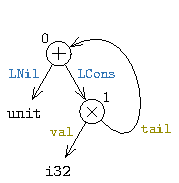
\includegraphics[scale=1.3]{chapters/figures/figTypeTreeList1.pdf}
\end{center}
\vspace{30px}
\caption{\label{fig:typetreelist1}\cons{List} = \cons{LNil} | \newline \cons{LCons}(\type{i32}, \type{List})}
\end{subfigure}%
&
\begin{subfigure}[b]{0.33\textwidth}
\begin{center}
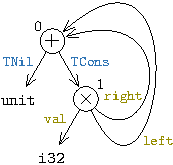
\includegraphics[scale=1.3]{chapters/figures/figTypeTreeTree1.pdf}
\end{center}
\vspace{35px}
\caption{\label{fig:typetreetree1}\cons{Tree} = \cons{TNil} | \newline \cons{TCons}(\type{i32}, \type{Tree}, \type{Tree})}
\end{subfigure}%
&
\begin{subfigure}[b]{0.33\textwidth}
\begin{center}
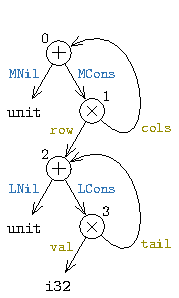
\includegraphics[scale=1.3]{chapters/figures/figTypeTreeMatrix1.pdf}
\end{center}
\caption{\label{fig:typetreematrix1}\cons{Matrix} = \cons{MNil} | \newline \cons{MCons}(\type{List}, \type{Matrix})}
\end{subfigure}%
\\
\end{tabular}
\caption{\label{fig:typetrees}Type trees for the ADTs \type{List}, \type{Tree} and \type{Matrix} respectively.}
\end{figure}

\Cref{fig:typetrees} shows the type trees for three ADTs \type{List}, \type{Tree}, and \type{Matrix} respectively.
In a type tree, each internal node represents either a product (\prodn{}) or a sum (\sumn{}) type constructor.
The leaf nodes are the scalar types.
Each outgoing edge of a \sumn{} node is associated with a data constructor of the corresponding ADT (i.e. \cons{LCons} for \type{List}).
Similarly, each outgoing edge of a \prodn{} node is associated with a field of the corresponding data constructor (i.e. \field{val} for \type{LCons}).
We assign integer indices to the internal nodes and use \ttedge{v}{label} to identify the edge outgoing at ${\tt v}$ associated with {\tt label},
where {\tt label} is either a data constructor or a field name.
The edges going outward from the root node are called {\em tree-edges} e.g., \ttedge{0}{LCons} and \ttedge{1}{val} in \cref{fig:typetreelist1}.
Edges that are not tree-edges, are called {\em back-edges} e.g., \ttedge{1}{cols} in \cref{fig:typetreematrix1}.
Every back-edge induces an unique simple cycle in the type tree representation.

\begin{figure}[H]
\begin{tabular}{@{}c@{}c@{}c@{}}
\begin{subfigure}[b]{0.30\textwidth}
\begin{center}
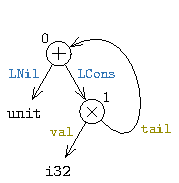
\includegraphics[scale=1.3]{chapters/figures/figTypeTreeList1.pdf}
\end{center}
\vspace{30px}
\caption{\label{fig:typetreelistpeel1} Canonical \type{List} ADT}
\end{subfigure}%
&
\begin{subfigure}[b]{0.33\textwidth}
\begin{center}
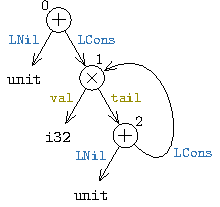
\includegraphics[scale=1.3]{chapters/figures/figTypeTreeList2.pdf}
\end{center}
\vspace{20px}
\caption{\label{fig:typetreelistpeel2} Peeled \type{List} ADT}
\end{subfigure}%
&
\begin{subfigure}[b]{0.33\textwidth}
\begin{center}
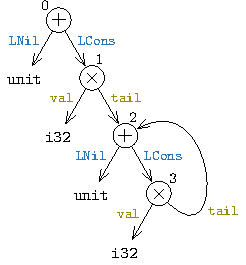
\includegraphics[scale=1.3]{chapters/figures/figTypeTreeList3.pdf}
\end{center}
\caption{\label{fig:typetreelistpeel3} Unrolled \type{List} ADT}
\end{subfigure}%
\\
\end{tabular}
\caption{\label{fig:typetreespeel}Three equivalent graphical representations for \type{List} ADT.
\Cref{fig:typetreelistpeel1} shows the graphical representation of the canonical form of \type{List}.
\Cref{fig:typetreelistpeel2} is obtained by peeling the {\em backedge} [2,1] in \cref{fig:typetreelistpeel1}.
\Cref{fig:typetreelistpeel3} is obtained by unrolling the backedge [2,1] in \cref{fig:typetreelistpeel1} or by
peeling the backedge [4,1] in \cref{fig:typetreelistpeel2} respectively.}
\end{figure}

Recall that types in \SpecL{} (and in IR also) follow equirecursive typing rules i.e. types
$\mu \alpha. T$ and $T[\mu \alpha. T/\alpha]$ in \typegrammar{} are {\em equal} types,
where $T[\mu \alpha. T/\alpha]$ represents the new type obtained by substituting all free
instances of $\alpha$ with $\mu \alpha. T$, and is defined as the {\em unfolding} of $\mu \alpha T$.
In general, under equirecursive typing, two types are equal iff their infinite expansions (through unfolding) are equal.
In the type tree representation, two types are equal iff their infinite expansions are equivalent.
An unfolding in the term representation corresponds to {\em unrolling} one iteration of a simple cycle in its type tree.
\Cref{fig:typetreespeel} shows three type trees for the \type{List} type.
\Cref{fig:typetreelistpeel1} corresponds to the canonical (intuitively the `smallest') type tree for the \type{List} type.
The type trees \cref{fig:typetreelistpeel2,fig:typetreelistpeel3} are obtained by {\em peeling} and unrolling
the back-edge \ttedge{1}{tail} (in \cref{fig:typetreelistpeel1}) respectively.
Peeling is a form of partial unrolling which only extracts the starting node of the cycle.
In practice, equality of two IR types (encoded in \typegrammar{}) can be reposed as syntactic
equality of their {\em canonical} forms.
In general, type trees may contain cycles (due to back-edges) and hence are not quite `trees'.
However, they represent the actual (possibly infinite) trees obtained through repeated unrolling of cycles.

\begin{figure}[H]
\begin{tabular}{cc}
\begin{subfigure}[b]{0.45\textwidth}
\begin{center}
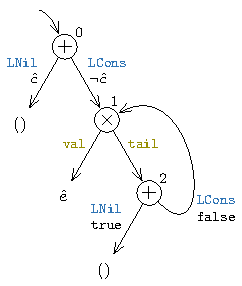
\includegraphics[scale=1.4]{chapters/figures/figValueTreeList1.pdf}
\end{center}
\caption{\label{fig:valuetreelist1}\sumIf{c} \sumThen{\cons{LNil}} \sumElse{\cons{LCons}(e, \cons{LNil})}}
\end{subfigure}%
&
\begin{tabular}{@{}c@{}}
\begin{subfigure}[b]{0.53\textwidth}
\begin{center}
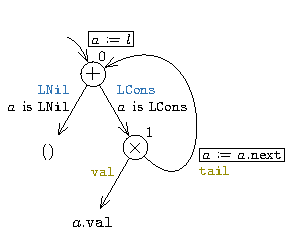
\includegraphics[scale=1.3]{chapters/figures/figValueTreeVarList.pdf}
\end{center}
\caption{\label{fig:valuetreevarlist}$l\ctype{List}$}
\end{subfigure}%
\\
\begin{subfigure}[b]{0.53\textwidth}
\begin{center}
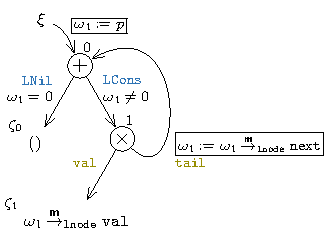
\includegraphics[scale=1.3]{chapters/figures/figValueTreeClist.pdf}
\end{center}
\caption{\label{fig:valuetreeclist}\lifted{list}{\mem{}}{lnode}{p}}
\end{subfigure}%
\\
\end{tabular}
\\
\end{tabular}
\caption{\label{fig:valuetrees}Value trees for three \type{List}-typed expressions.}
\end{figure}

With type trees out of the way, we are ready to present their value analogue called `value trees'.
\Cref{fig:valuetrees} shows the value trees for three \type{List} expressions.
Note that, all three value trees are isomorphic (i.e. identical structures) to one of the
\type{List} type trees shown in \cref{fig:typetreespeel}, e.g.,
\cref{fig:valuetreelist1} is isomorphic to \cref{fig:typetreelistpeel2}.
In general, a value tree $\mathcal{V}(e)$ (for the expression $e$ of type $t$) is isomorphic to a
type tree $\mathcal{T}(t)$ with the following distinctions:

\begin{enumerate}
\item Similar to $\mathcal{T}(t)$, each internal node is either a \sumn{} or a \prodn{} node.
\item Instead of a scalar type $t$, each leaf node in $\mathcal{V}(e)$ contains an expression
of type $t$.
\item In addition to a data constructor, each edge originating at a \sumn{} node also contains
an edge condition expression. We identify such an edge with \vtedge{i}{V}{c}, where {\tt i} is the index of
the sum node, $V$ is the data constructor and $c$ is the edge condition.
The set of edge conditions for all outgoing edges at a \sumn{} node must be mutually exclusive and exhaustive.
\item In addition to a field name, each edge originating at a product (\circled{$\times$}) node also contains
a transfer function. We identify such an edge with \vtedge{i}{f}{\omega}, where {\tt i} is the index of
the product node, $f$ is the field name and $\omega$ is the transfer function.
\item $\mathcal{V}(e)$ also contains a special node (called the {\em entry node}), and a special edge
(called the {\em entry edge}) from the entry node to the root node. The entry edge contains a transfer
function. We often omit the entry node in figures.
\end{enumerate}

Intuitively, a value tree simultaneously represents the value of the expression as well as a program
similar to its deconstruction program.
Next, we give an algorithm to convert an expression $e$ to its value tree representation $\mathcal{V}(e)$
and list its properties and applications in the context of our proof discharge algorithm.

\subsection{Conversion of Expressions to their Value Graphs}

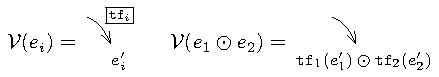
\includegraphics[scale=1.3]{chapters/figures/figValueTreeConvScalar.pdf}

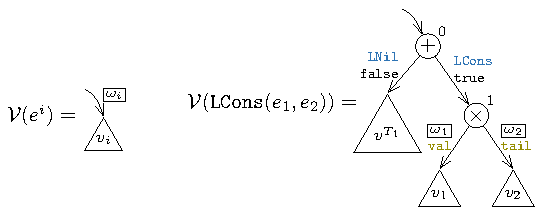
\includegraphics[scale=1.3]{chapters/figures/figValueTreeConvCons.pdf}

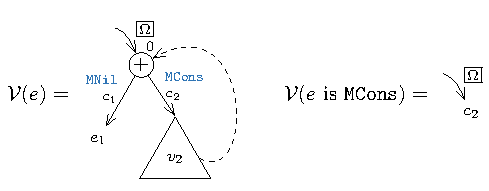
\includegraphics[scale=1.3]{chapters/figures/figValueTreeConvSumIs.pdf}

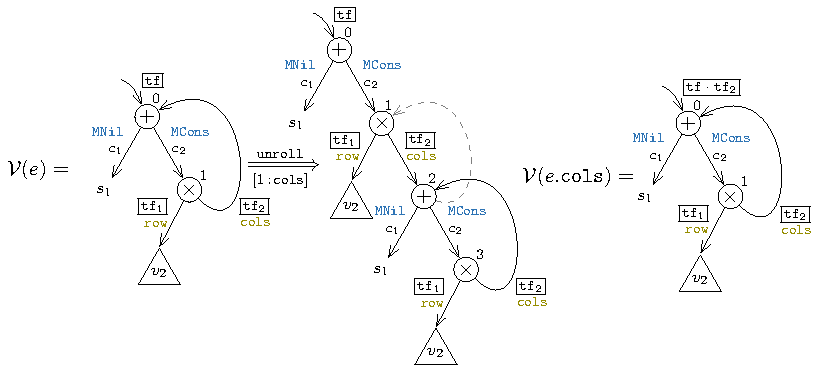
\includegraphics[scale=1.3]{chapters/figures/figValueTreeConvProdAccess.pdf}

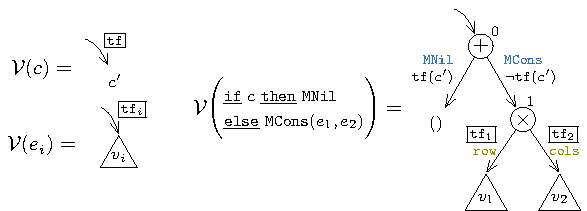
\includegraphics[scale=1.3]{chapters/figures/figValueTreeConvIte.pdf}

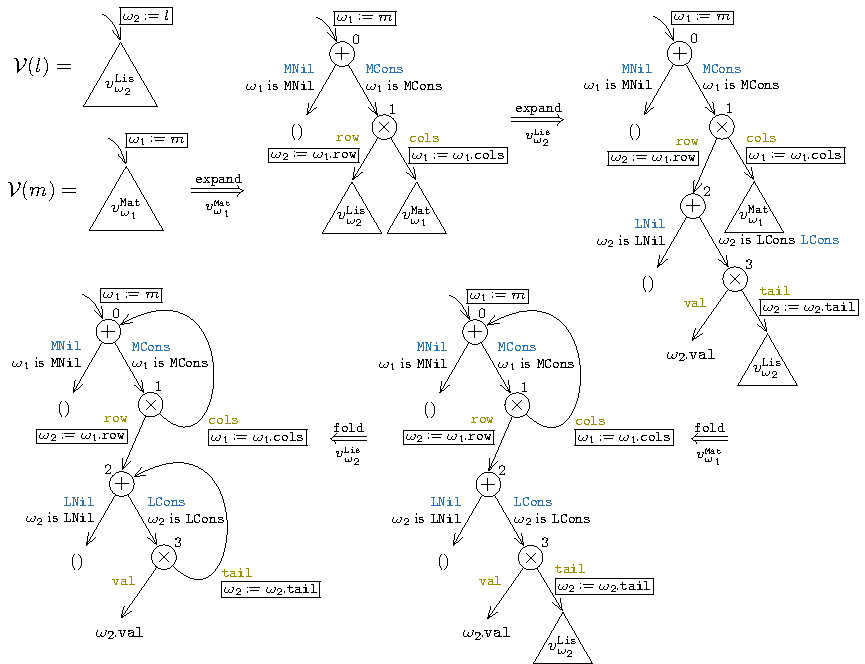
\includegraphics[scale=1.3]{chapters/figures/figValueTreeConvVar.pdf}

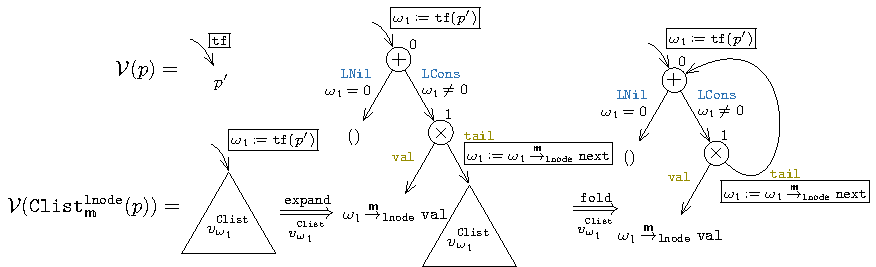
\includegraphics[scale=1.3]{chapters/figures/figValueTreeConvLift.pdf}

\subsection{Applications of Value Graphs}

\subsubsection{Approximations of a Recursive Relation}

\subsubsection{Bisimilarity of Deconstruction Programs}

We give an algorithm for converting an arbitrary expression $e$ to its value tree.
Next, we reformulate multiple procedures related to our proof discharge algorithm
in terms of the value trees directly.

today: draw the figures for all conversions first
then write a first draft

tomorrow: draw the figures for decomposition, the 2 deconstruction programs, their unified forms and
points-to analysis on them


then go straight into the conversion algorithm
quite easy for most
some time on if-then-else
some times on the variable + lifting constructor
straight into recursive relations
decomposition
approximations
then deconstruction program alternative
unification using the example
give the same example with points-to analysis on it
write the final algorithm
DONE
(will need like 5-6 days to write all this out with figures)
but for now, i can atleast try to do as much as possible so sir can start to review it
